\documentclass{scrartcl}

\usepackage{amssymb}
\usepackage{amsmath}
\usepackage{tikz}
\usetikzlibrary{calc,intersections,through,backgrounds,patterns}
\usetikzlibrary{decorations.text, decorations.markings, fit, arrows, arrows.meta}

%via Easley & Kleinberg - Networks, Crowds, and Markets; Reasoning about a Highly Connected World, pp. 208-9

\begin{document}
	
	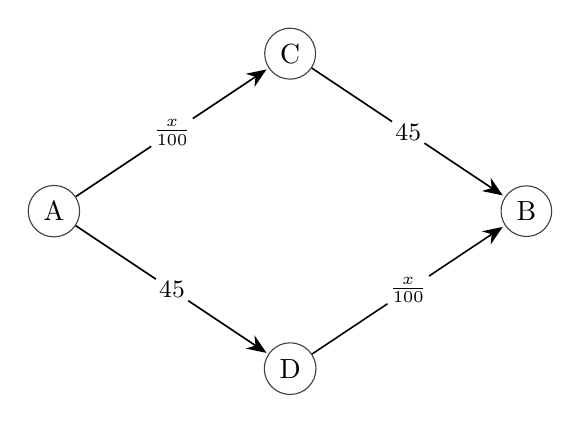
\begin{tikzpicture}
	%arrows
	\draw[-{Stealth[length=2.5mm,width=2mm]},semithick] (-3,0)--(-0.3,1.8);		%A--C
	\draw[-{Stealth[length=2.5mm,width=2mm]},semithick] (-3,0)--(-0.3,-1.8);	%A--D
	\draw[-{Stealth[length=2.5mm,width=2mm]},semithick] (0,2)--(2.7,0.2);		%C--B
	\draw[-{Stealth[length=2.5mm,width=2mm]},semithick] (0,-2)--(2.7,-0.2);		%D--B
	
	%circles
	\filldraw (-3,0)node[circle,inner sep=3pt,draw=darkgray,fill=white] {A};
	\filldraw (3,0) node[circle,inner sep=3pt,draw=darkgray,fill=white] {B};
	\filldraw (0,2) node[circle,inner sep=3pt,draw=darkgray,fill=white] {C};
	\filldraw (0,-2)node[circle,inner sep=3pt,draw=darkgray,fill=white] {D};
	
	%manual fill
	\fill[white] (-1.5,1) circle (9pt); 
	\fill[white] (-1.5,-1)circle (7pt); 
	\fill[white] (1.5,1)  circle (7pt); 
	\fill[white] (1.5,-1) circle (9pt);
	
	%outer labels
	\node at (-1.5,1) {{\small $\frac{x}{100}$}};
	\node at (-1.5,-1){{\small $45$}};
	\node at (1.5,1)  {{\small $45$}};
	\node at (1.5,-1) {{\small $\frac{x}{100}$}};
	
	%\draw[help lines] (-3,-2) grid (3,2);
	\end{tikzpicture}
	
	
	\vspace{2cm}
	
	
	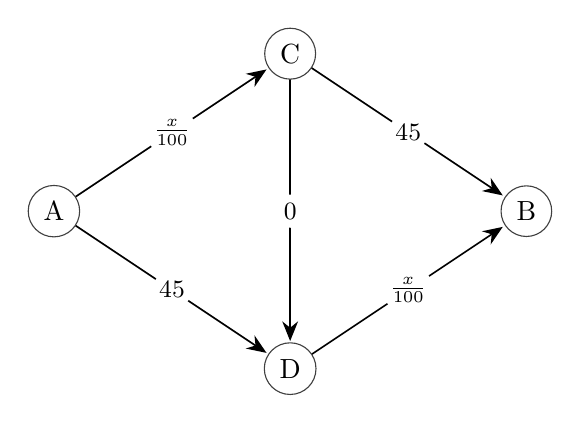
\begin{tikzpicture}
	%arrows
	\draw[-{Stealth[length=2.5mm,width=2mm]},semithick] (-3,0)--(-0.3,1.8);		%A--C
	\draw[-{Stealth[length=2.5mm,width=2mm]},semithick] (-3,0)--(-0.3,-1.8);	%A--D
	\draw[-{Stealth[length=2.5mm,width=2mm]},semithick] (0,2)--(2.7,0.2);		%C--B
	\draw[-{Stealth[length=2.5mm,width=2mm]},semithick] (0,-2)--(2.7,-0.2);		%D--B
	\draw[-{Stealth[length=2.5mm,width=2mm]},semithick] (0,2)--(0,-1.65);		%C--D
	
	%circles
	\filldraw (-3,0)node[circle,inner sep=3pt,draw=darkgray,fill=white] {A};
	\filldraw (3,0) node[circle,inner sep=3pt,draw=darkgray,fill=white] {B};
	\filldraw (0,2) node[circle,inner sep=3pt,draw=darkgray,fill=white] {C};
	\filldraw (0,-2)node[circle,inner sep=3pt,draw=darkgray,fill=white] {D};
	
	%manual fill
	\fill[white] (-1.5,1) circle (9pt); 
	\fill[white] (-1.5,-1)circle (7pt); 
	\fill[white] (1.5,1)  circle (7pt); 
	\fill[white] (1.5,-1) circle (9pt);
	\fill[white] (0,0)    circle (6pt); 
	
	%outer labels
	\node at (-1.5,1) {{\small $\frac{x}{100}$}};
	\node at (-1.5,-1){{\small $45$}};
	\node at (1.5,1)  {{\small $45$}};
	\node at (1.5,-1) {{\small $\frac{x}{100}$}};
	\node at (0,0)    {{\small $0$}};
	
	%\draw[help lines] (-3,-2) grid (3,2);
	\end{tikzpicture}
	
\end{document}